%
%\addtocontents{toc}{\newpage}
\chapter{Principal Component Analysis}
\label{cpt:pca}

Principal Component Analysis (PCA) is a powerful tool that extracts the most significant features from a given dataset.  Given a set of images $I$ and an integer $k>0$, PCA projects $I$ onto the $k$ orthogonal basis vectors that best approximate $I$.  Each image can be approximated by a linear combination of the basis vectors.

\section{PCA Math}

Given a set of $n$ $w$-by-$h$ images $I$, we create an $n$-by-$(w*h)$ matrix $D$, where each column is an image flattened into a vector with the mean image subtracted from it.  We can now use a linear algebra technique called singular value decomposition (SVD) to solve for matrices $U, S, V$ such that $$M \approx USV.$$where $U$ contains the $k$ orthogonal basis images as its columns, $S$ is a diagonal matrix which contains the weights, or singular values, of each feature vector, and $V$ contains the coefficients of the linear combination of basis vectors that best approximates each vector in $D$.

To reconstruct an image vector $I_x$, we convert it to a vector $I_{x-mean} = I_x - I_{mean}$, and we can say $$I_{x-mean} \approx I_{reconstructed} = USV_x$$where $V_x$ is the vector of coefficients corresponding to $I_x$.  If $k < n$, our reconstruction is not guaranteed to be perfect, but as $k$ approaches $n$, the reconstruction gets better, as shown in Figure \ref{fig:pcaIntro}.  The reconstruction error, or residual, can be calculated as $$I_{residual} = I_{x-mean} - I_{reconstructed}$$


\begin{figure}[t]
	\centering
	\subfigure[]{
		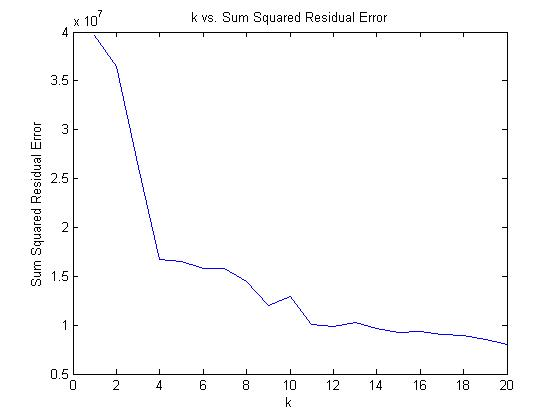
\includegraphics[width=.4\textwidth]{figures/pcaIntroPlot.jpg}
	\label{fig:pcaIntroPlot}
	}
	\subfigure[]{
		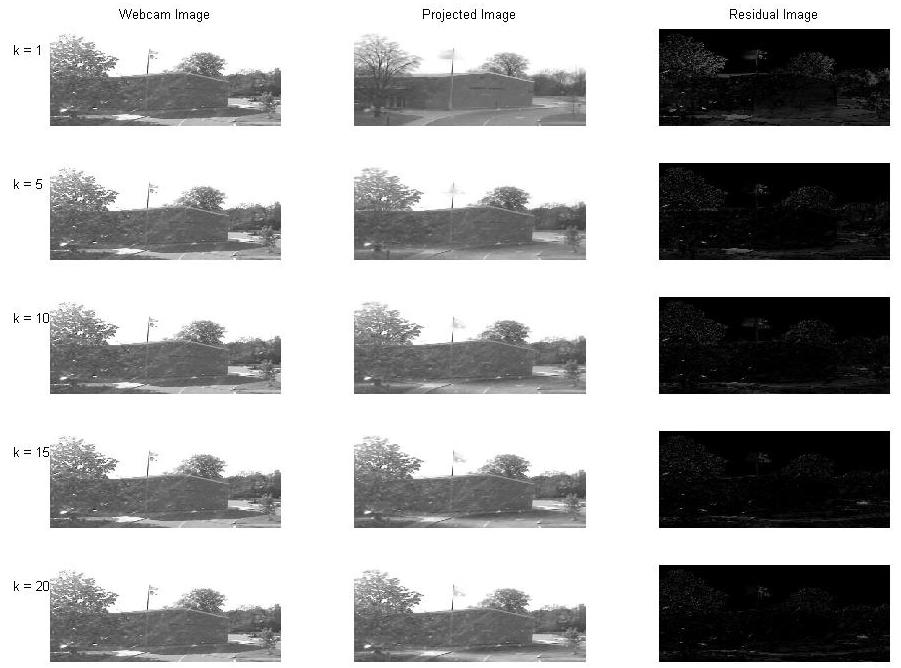
\includegraphics[width=.55\textwidth]{figures/pcaIntroFigs.jpg}
	\label{fig:pcaIntroFigs}
	}
	
		\caption[PCA reconstruction and residual images for different values of k]{Figure \ref{fig:pcaIntroPlot} plots the sum squared residual error for reconstruction of a webcam image for values of $k$ from 0 to 50, and $n = 189$.  When $k = 0$, the reconstruction is simply the mean image.  Figure \ref{fig:pcaIntroFigs} shows the image, the reconstruction, and residual for $k = \{0, 1, 10, 50\}$.  Notice that we start to model the cars at $k=10$ and get a great approximation at $k=50$.}
\label{fig:pcaIntro}
\end{figure}

In situations where dataset sizes conflict with memory constraints, we can use a modified algorithm called Incremental PCA, which allows allows us to iteratively update our matrices $U, S, V$ for new images\cite{Brand02incrementalsingular}.